\subsection{Measurement Scope \& Datasets}
\label{cloud-measure-background}


\begin{figure}[t]
\centering
\begin{subfigure}[b]{0.20\textwidth}
    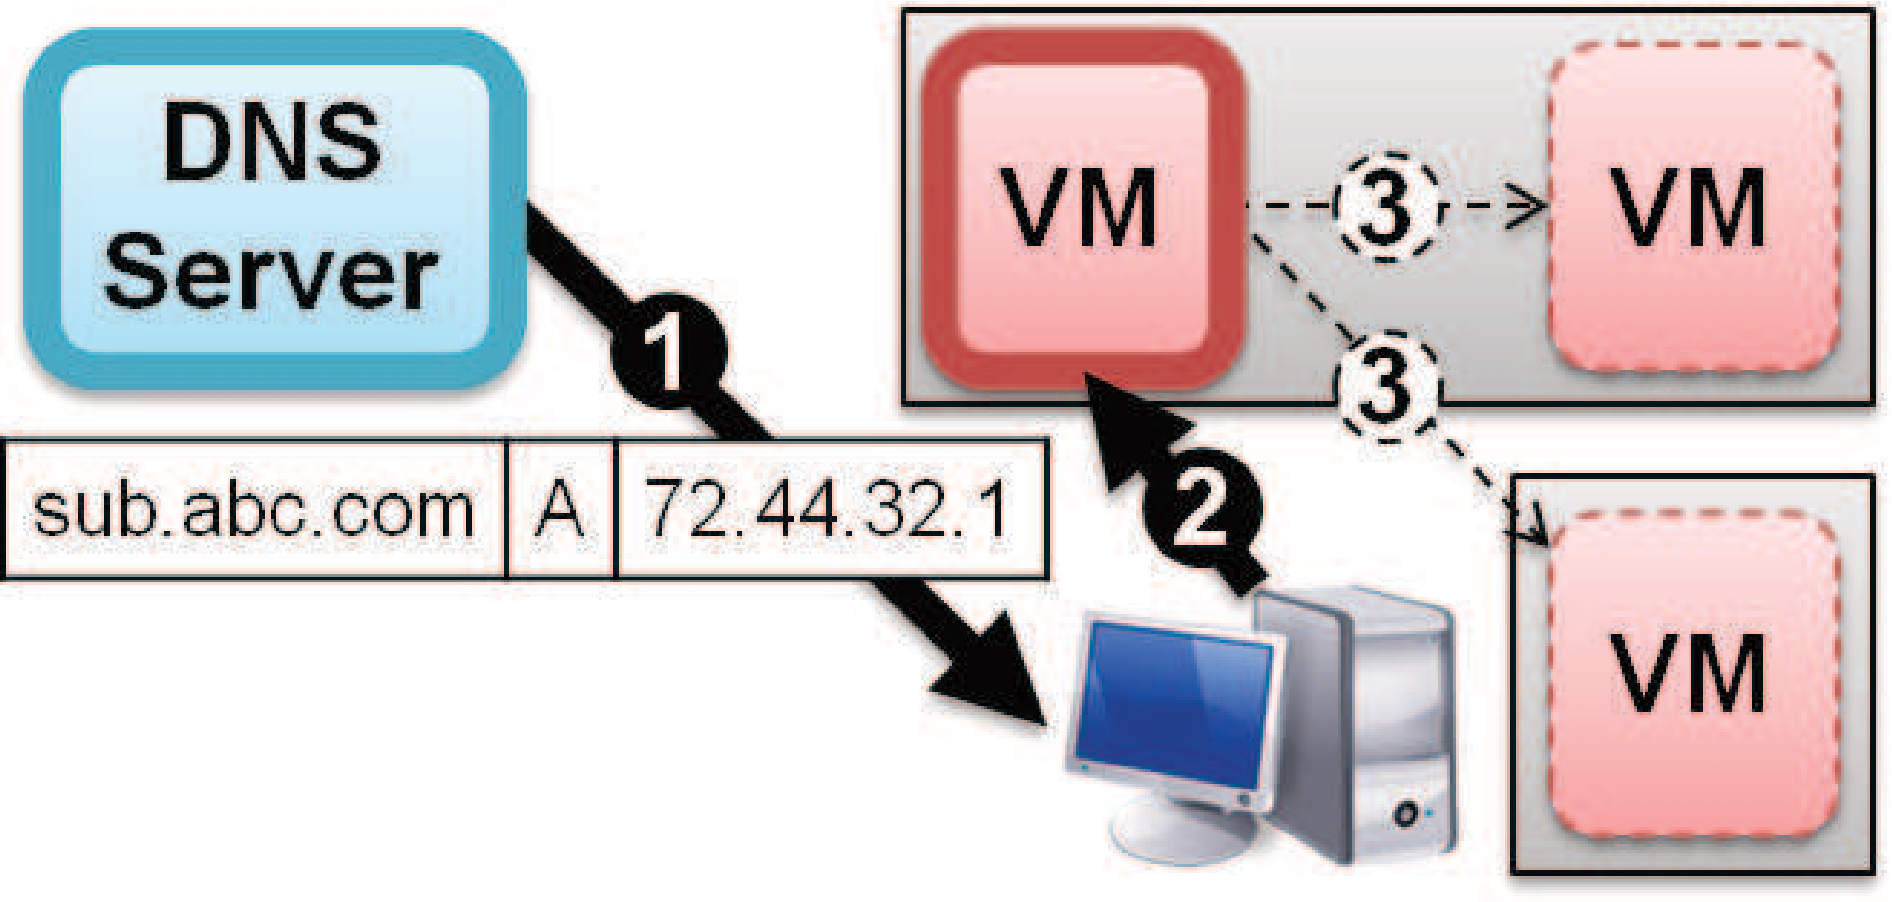
\includegraphics[width=\textwidth]{figures/cloudmeasure/imag_sec2/ec2_vm.pdf}
    \caption{P1: VM front end}
    \label{fig:ec2_vm}
\end{subfigure}
\hspace{0.03\columnwidth}
\begin{subfigure}[b]{0.3\textwidth}
    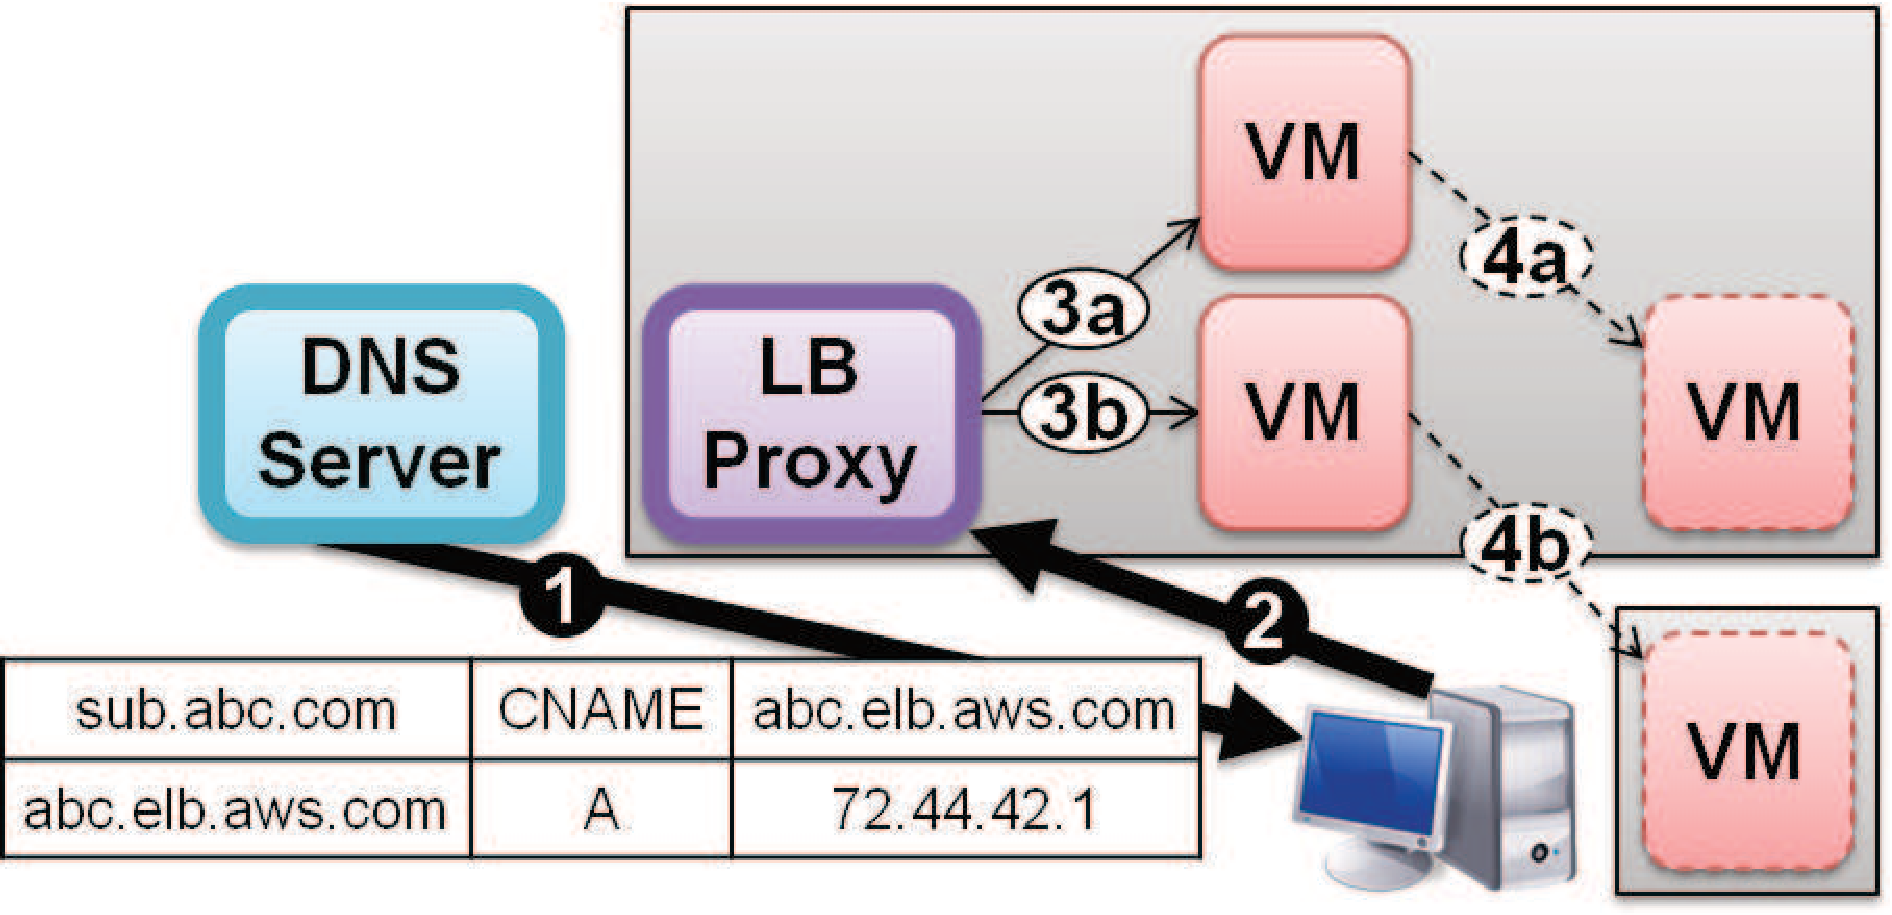
\includegraphics[width=\textwidth]{figures/cloudmeasure/imag_sec2/ec2_elb.pdf}
    \caption{P2: Load balancer front end}
    \label{fig:ec2_elb}
\end{subfigure}

\begin{subfigure}[b]{0.20\textwidth}
    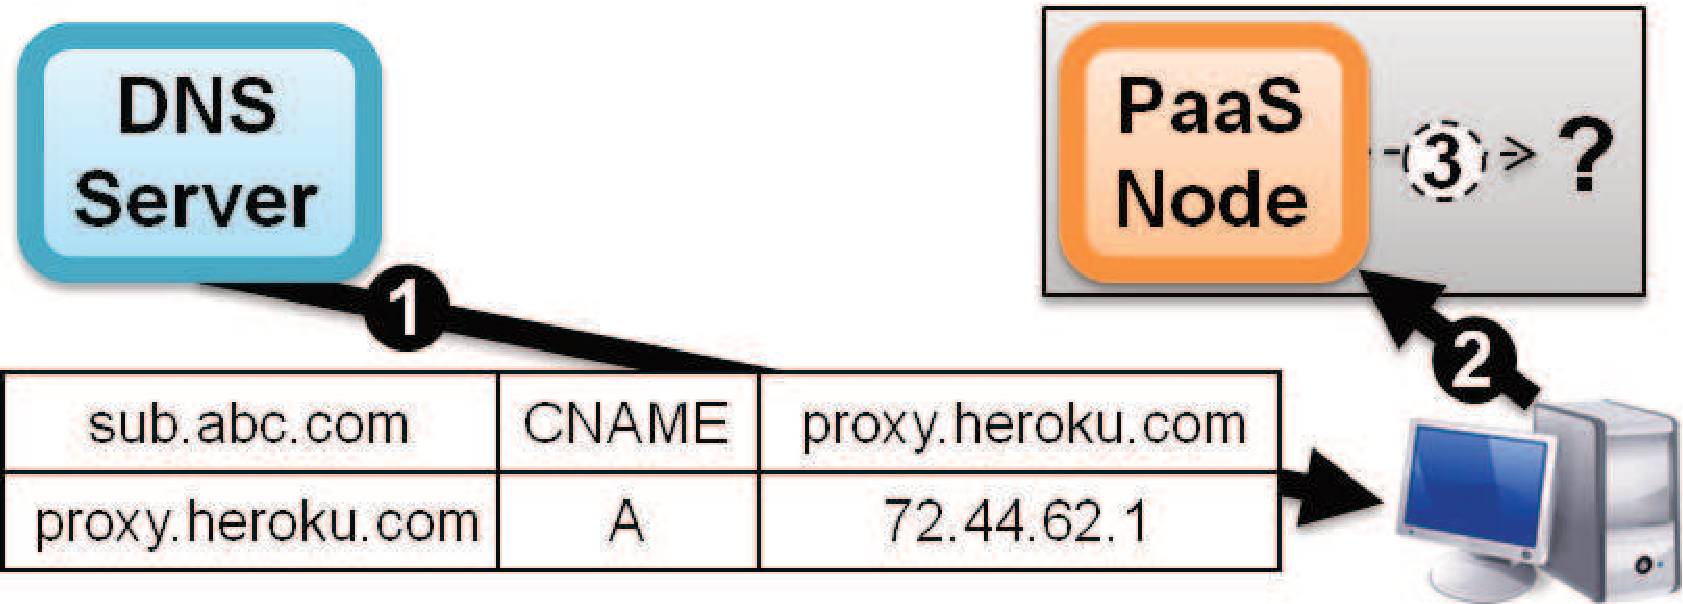
\includegraphics[width=\textwidth]{figures/cloudmeasure/imag_sec2/ec2_heroku.pdf}
    \caption{P3: PaaS front end}
    \label{fig:ec2_paas}
\end{subfigure}
\hspace{0.03\columnwidth}
\begin{subfigure}[b]{0.30\textwidth}
    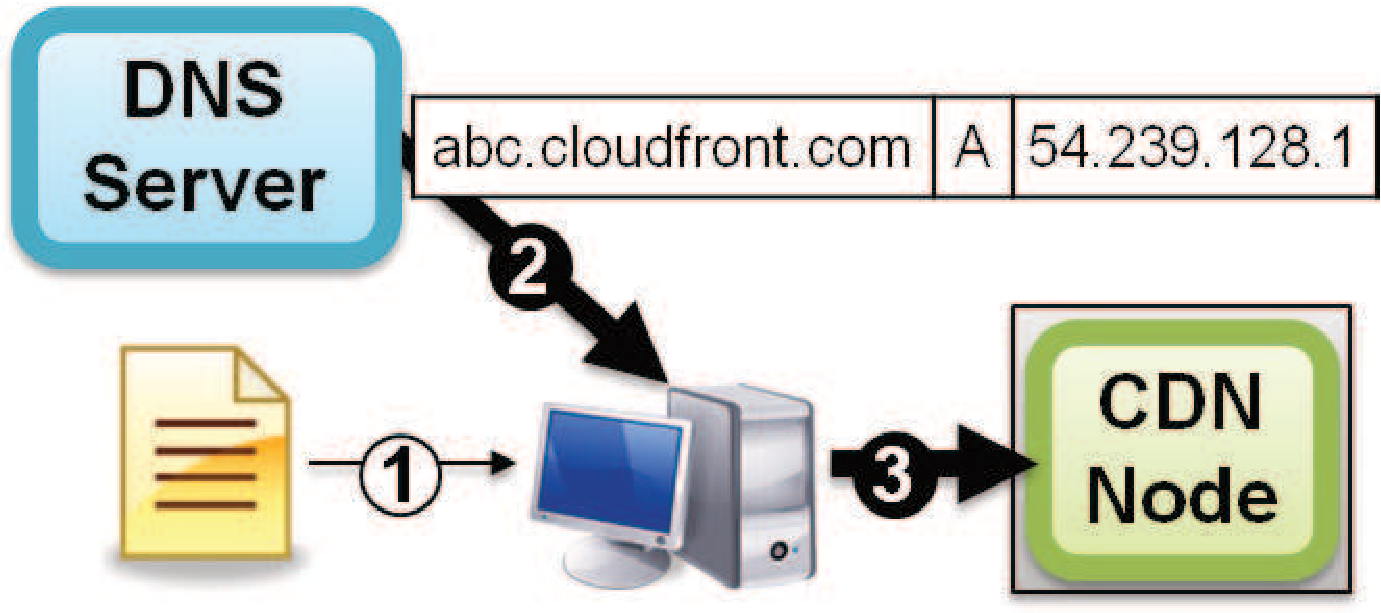
\includegraphics[width=\textwidth]{figures/cloudmeasure/imag_sec2/ec2_cdn.pdf}
    \caption{P4: Leverage CDN}
    \label{fig:ec2_cdn}
\end{subfigure}

\caption{Deployment patterns for web services.}
\label{fig:ec2_models}

\end{figure}


Public IaaS clouds, such as Amazon EC2, Windows Azure, and Rackspace,
allow tenants to dynamically rent virtual machine (VM) instances with
varying CPU, network, and storage capacity. Cloud tenants have the
option of renting VMs in one or more geographically distinct
data centers, or {\em regions}. Some clouds, such as EC2,
further divide these regions into multiple distinct availability {\em
  zones}. Each zone has separate compute and power
infrastructure to make certain failure modes zone-specific and to
allow cloud tenants to replicate their deployments across
multiple zones for smooth fail-over.

Beyond simple VMs, IaaS providers, as well as third parties, offer a
wide-range of value-added features: load balancers (e.g., Amazon
Elastic Load Balancer and Azure Traffic Manager),
plat\-form-as-a-service environments (e.g., Amazon Elastic
Beanstalk, Heroku, and Azure Cloud Services), content-distribution networks
(e.g., Amazon CloudFront and Azure Media Services), DNS hosting (e.g.,
Amazon route53), etc. The result is a complex ecosystem of
interdependent systems operating at multiple layers of abstraction,
and, in turn, a large variety of possible deployment patterns for
cloud tenants. In this paper, we study four popular deployment patterns. We
describe these using a series of examples.

In \figref{fig:ec2_models}, we show the steps involved in a client
accessing an EC2-hosted web service that is using one or more of the
aforementioned features. When a client wants to access a web service,
it first performs a DNS lookup of the service's domain name.  The
response may contain an IP address associated with a VM (deployment
pattern {\em P1}), a load balancer ({\em P2}), or a
platform-as-a-service (PaaS) node ({\em P3}).
With {\em P2}, the client request is subsequently directed to a
VM\footnote{Or PaaS
  nodes, as is done by Amazon Elastic Beanstalk and Azure Traffic
  Manager.}. Tenants using {\em P1}--{\em P3} may also rely on
additional VMs or systems (dashed lines) to handle a
client's request; these additional components may or may not be in the
same region or availability zone (indicated by the gray boxes). An
object returned to a client (e.g., a web page) may sometimes require
the client to obtain additional objects (e.g., a video) from a
content-distribution network ({\em P4}).

We focus on studying the front end portions of web
service deployments within the above four deployment patterns (indicated by 
the thicker lines in \figref{fig:ec2_models}). These
portions are encountered within the initial few steps of a client
making a request. We leave an exploration of deployment/usage patterns
covering the later steps (e.g. back-end processing) for future work.


\subsubsection{Datasets}
\label{cloud-measure-datasets}

We use two primary datasets: ({\em i}) a list of cloud-using
subdomains derived from Alexa's list of the top 1 million websites,
and ({\em ii}) packet traces captured at the border of the
UW-Madison campus network. Both datasets leverage the fact that EC2~\cite{ec2iprange}
and Azure~\cite{azureiprange} publish a list of the public IPv4
address ranges associated with their IaaS cloud offerings. Below, we
provide details on our \alexadata and \capturedata datasets. We
augment these data sets with additional traces and active measurements
to aid specific analyses; we describe these at the appropriate places
in subsequent sections.


\tightparagraph{Top Cloud-Using Subdomains Dataset}
Our first dataset is a list of subdomains which use EC2 or Azure and are 
associated with domains on Alexa's list of the top 1 million
websites~\cite{alex_topdomains}. We consider a subdomain to use EC2 or Azure if a
DNS record for that subdomain contains an IP address that falls within EC2 or
Azure's public IP address ranges. 

To construct this dataset, we first identified the subdomains associated with
each domain on Alexa's list of the top 1 million websites.  We started
with Alexa's top 1 million list from Feburary 6, 2013 and attempted to issue
a DNS zone transfer (i.e., a DNS query of type AXFR) for each domain on the
list.  The query was successful for only about 80K of the domains.  For the
remaining domains, we used dnsmap~\cite{dnsmap} to identify subdomains by
brute-force. Dnsmap uses a pre-defined word list, which we augmented with the
word list from knock~\cite{knock}, to construct potential subdomain names.
Dnsmap then runs DNS queries to check if the potential subdomains actually 
exist. This brute-force approach misses some subdomains,
but it allows us to provide a lower bound on the number of subdomains which 
use public IaaS clouds and explore the deployment patterns of these known 
cloud-using subdomains.
We distributed this task to 150 globally-distributed PlanetLab
nodes, producing a list of 34 million valid subdomains.

To limit the list of subdomains to cloud-using subdomains, we performed a series of
DNS lookups using the UNIX dig utility. We first performed a single
DNS lookup from one PlanetLab node (chosen from our set of 150 nodes)
for each subdomain. If the DNS record contained an IP address within
EC2 or Azure's public IP ranges\footnote{We assume the IP address ranges 
published by EC2 and Azure are relatively complete.}, we included it on our 
list of the top
cloud-using subdomains. This resulted in a list of 713K cloud-using
subdomains. We then performed a DNS lookup for each of the cloud-using
subdomains on every node in a set of 200 globally-distributed
PlanetLab nodes. \figref{fig:nodes_deploy} shows the geographic location of 
these PlanetLab nodes, which are spread across North America, South America,
Europe, Asia, and Australia.
The queries were performed March 27-29,
2013. These distributed DNS queries help ensure that we gather a
comprehensive set of DNS records for each cloud-using subdomain and
capture any geo-location-specific cloud usage.

We refer to the list of cloud-using subdomains, and their associated
DNS records, as the \alexadata dataset. 


 \begin{figure}[tb]
 \centering
 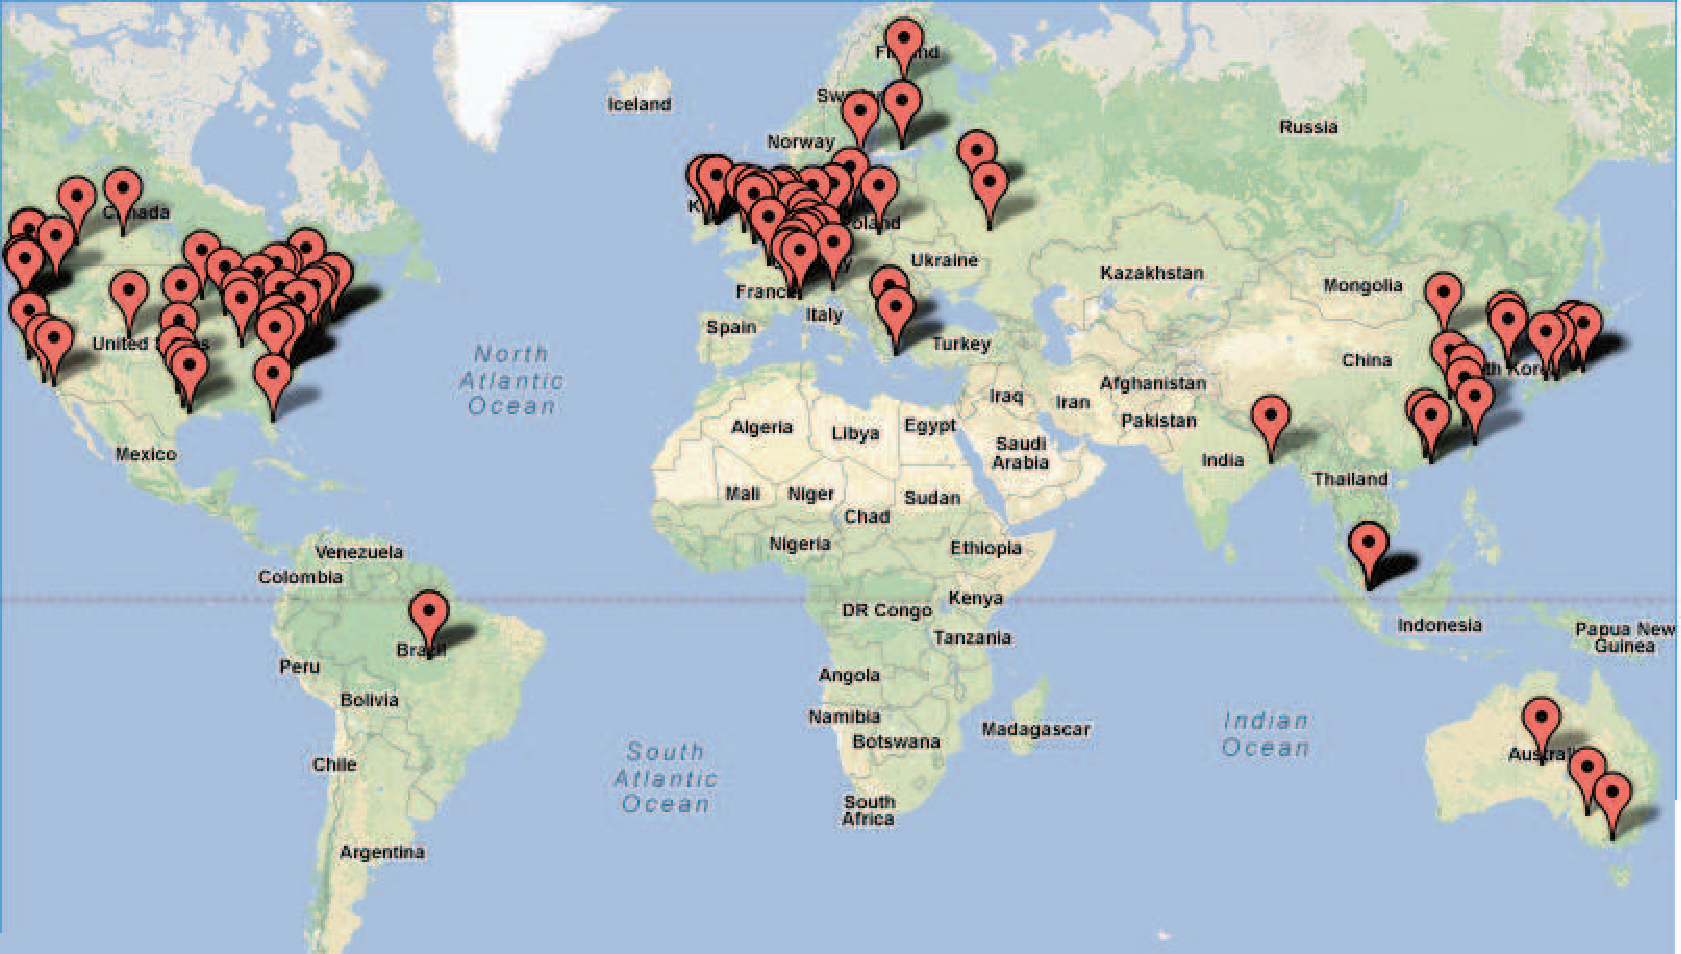
\includegraphics[width=0.55\columnwidth]{figures/cloudmeasure/imag_sec2/nodes_deploy.pdf}
 \caption{PlanetLab nodes used for DNS lookups\label{fig:nodes_deploy}}
 \end{figure}

%%%%%%%%%%%%%%%%%%%%%%%%%%%%%%%%%%%%%%%%%%%%%%%%%%%%%%%%%%%%%%%%%%%%%%%%%%%%%

\tightparagraph{Packet Capture Dataset} Our second primary dataset is a
series of packet traces captured at the border of the University of
Wisconsin-Madison campus network\footnote{The university has seven /24 IP blocks and one /16
IP block}. We captured full IP packets whose source or destination IP
address fell within the public address ranges published by EC2 and
Azure. The capture was performed from Tuesday, June 26 to Monday, July
2, 2012 giving us a full week of traffic and a total of 1.4TB of data.
The total Internet traffic averaged approximately 7Gbps during the capture,
with about 1\% of the traffic going to/coming from EC2 or Azure. Due to the
relatively low rate of traffic being captured, no loss occurred during the
capture process (according to tcpdump and counters reported by the border
router). 
To protect user privacy, we anonymized the IP addresses of clients
within the university network, and we only report aggregate
statistics.

Since our traces contain full packets, we were able to perform an
in-depth analysis of network and transport layer information (e.g., IP
addresses, protocols, ports), application layer information (e.g.,
HTTP hostnames, HTTP content-type, HTTPS certificates), and packet
payloads. We extracted relevant information from the traces using
Bro~\cite{paxson1998bro}, a network monitoring and traffic analysis
tool. We refer to these traces as the
\captureonedata dataset.



%%%%%%%%%%%%%%%%%%%%%%%%%%%%%%%%%%%%%%%%%%%%%%%%%%%%%%%%%%%%%%%%%%%%%%%%%%%%%


